\section{Results}
\label{sec:results}

\aim{Make similar plots for Brier and CDE Loss.}

\aim{Consense these images into fewer plots.}

\aim{Write descriptions of tests}

\subsection{Mock classifier systematics}
\label{sec:mockresults}

\begin{figure}
	\begin{center}
		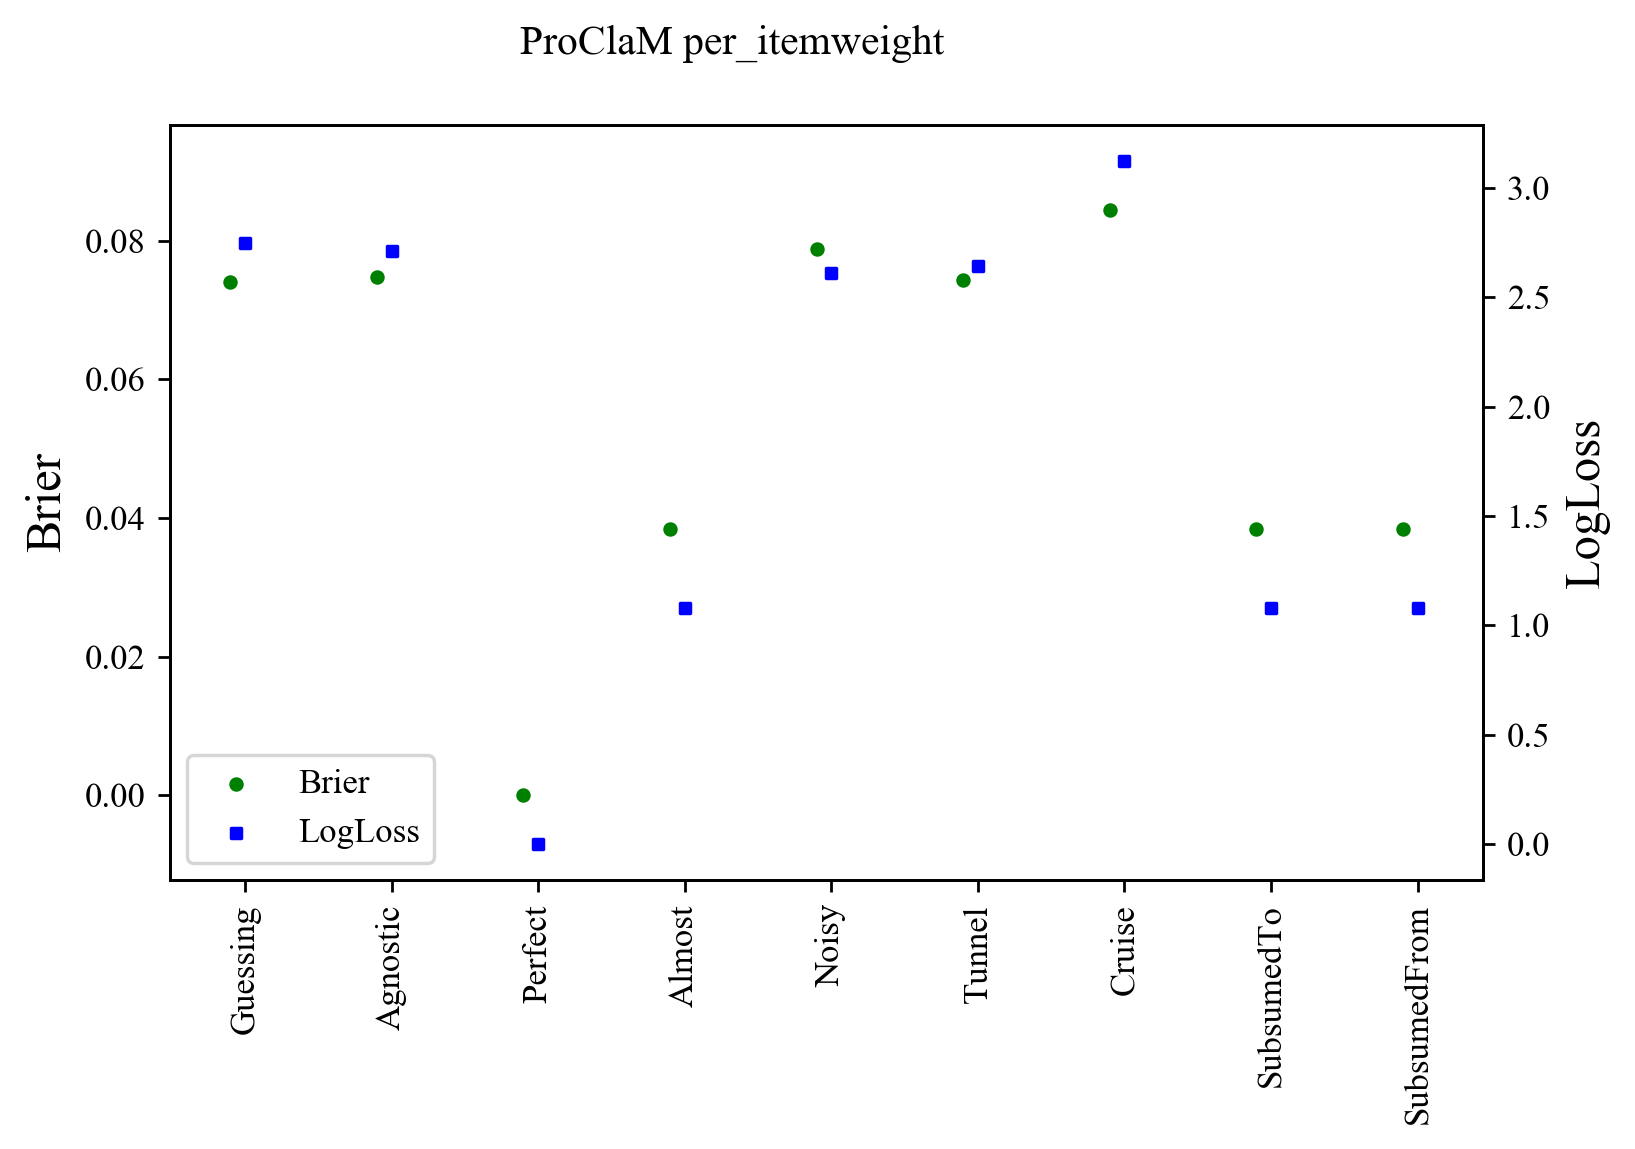
\includegraphics[width=0.5\textwidth]{./fig/multi_metric_per_item.png}
		\caption{}
		\label{fig:plasticc_per_item}
	\end{center}
\end{figure}

\begin{figure}
	\begin{center}
		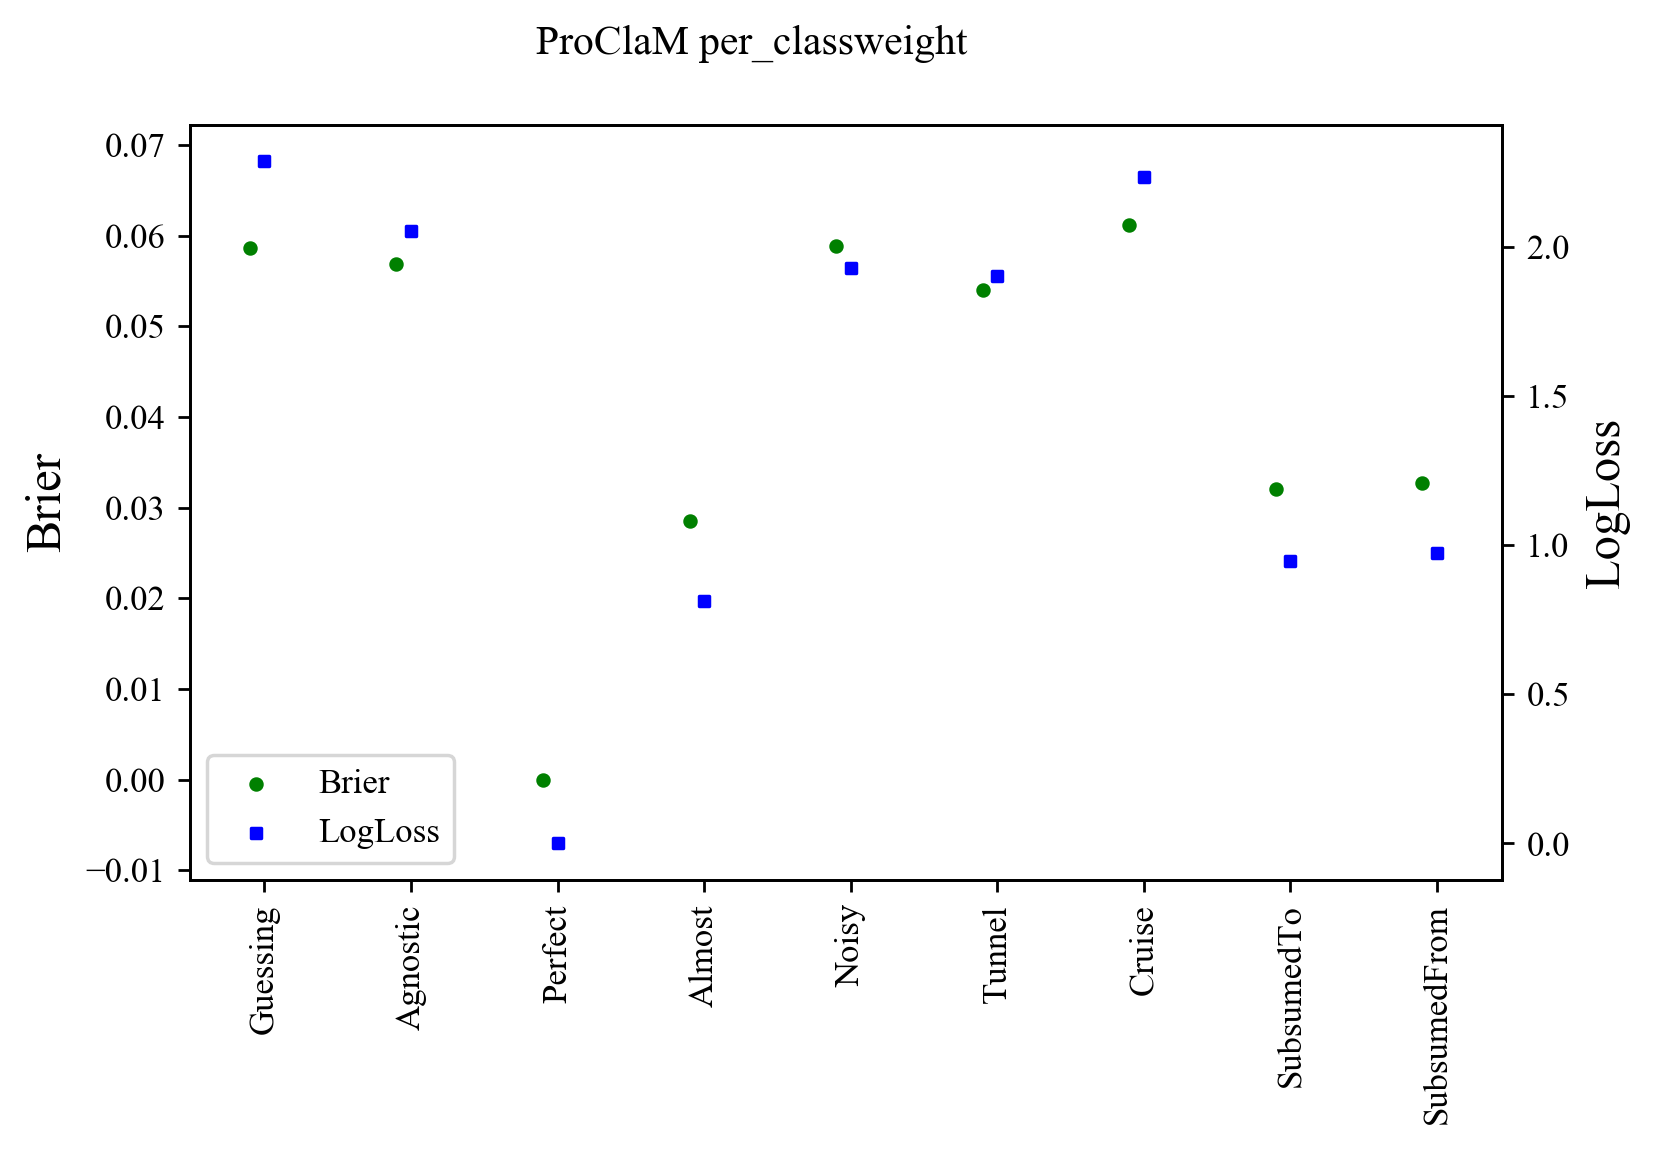
\includegraphics[width=0.5\textwidth]{./fig/multi_metric_per_class.png}
		\caption{}
		\label{fig:plasticc_per_class}
	\end{center}
\end{figure}

\begin{figure}
	\begin{center}
		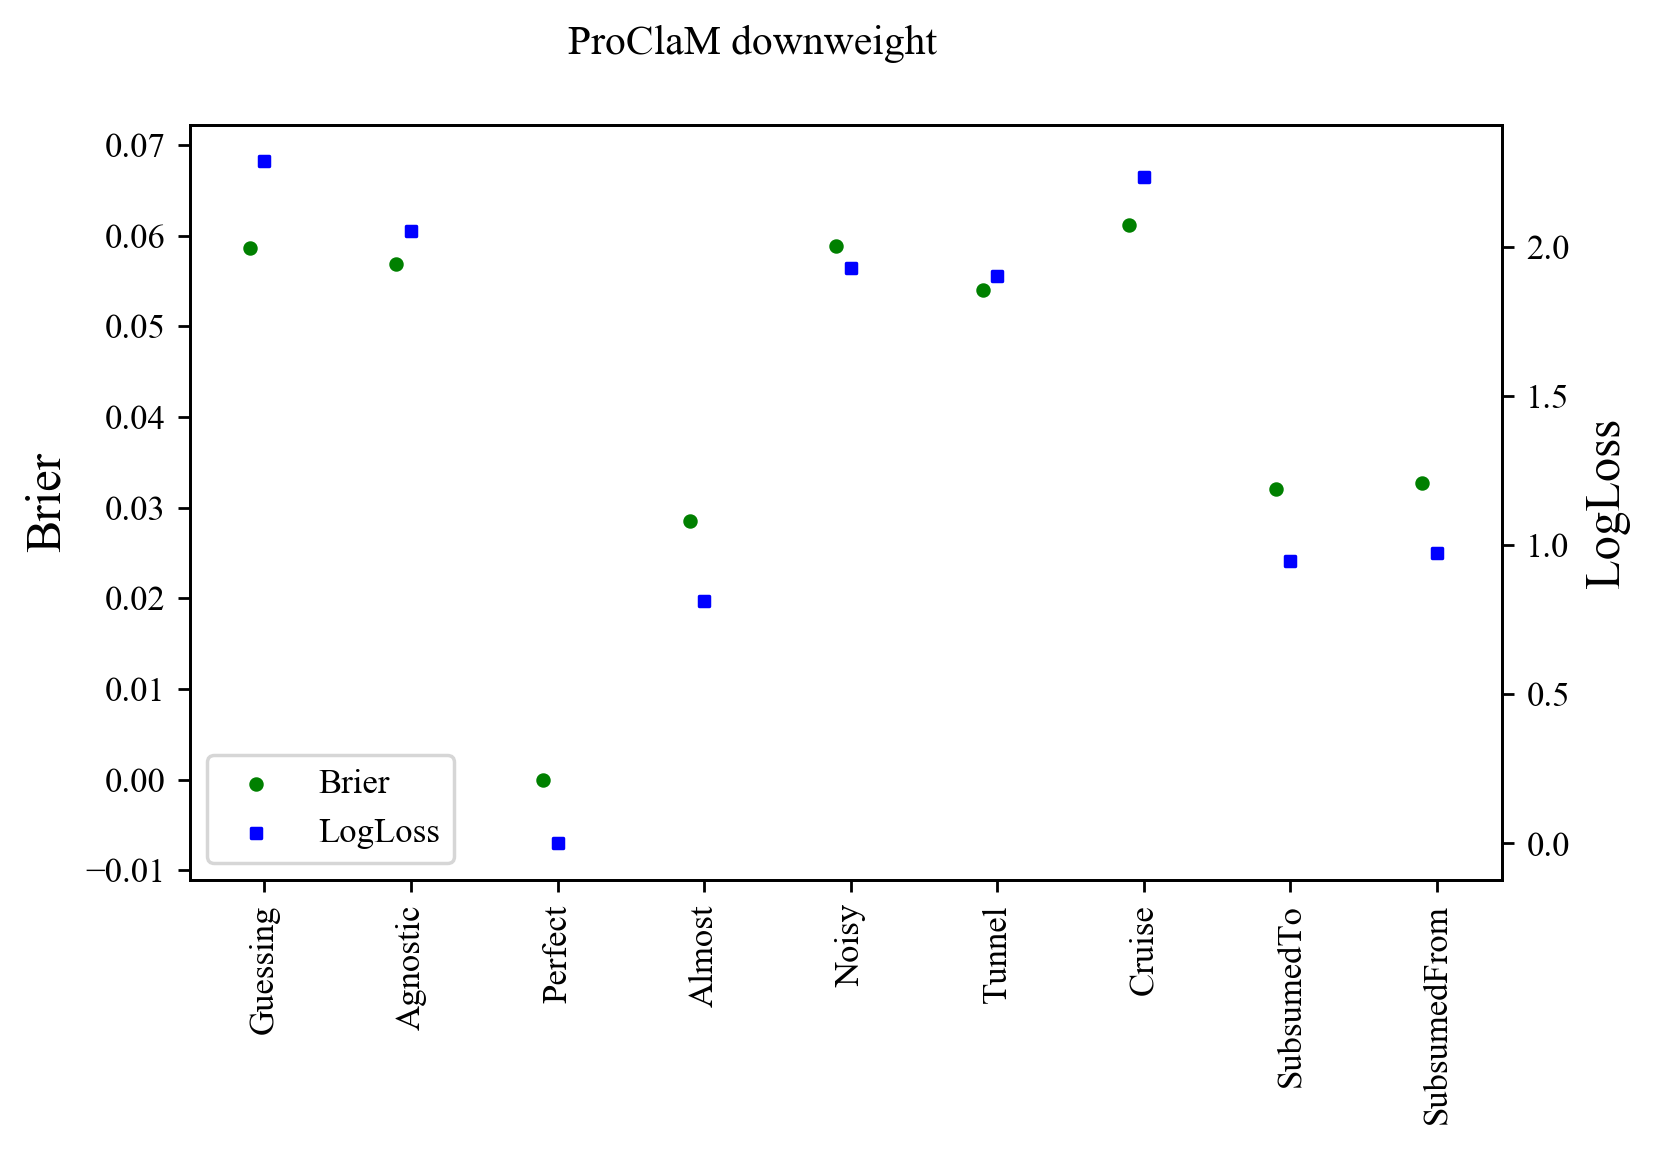
\includegraphics[width=0.5\textwidth]{./fig/multi_metric_down.png}
		\caption{}
		\label{fig:plasticc_down}
	\end{center}
\end{figure}

\begin{figure}
	\begin{center}
		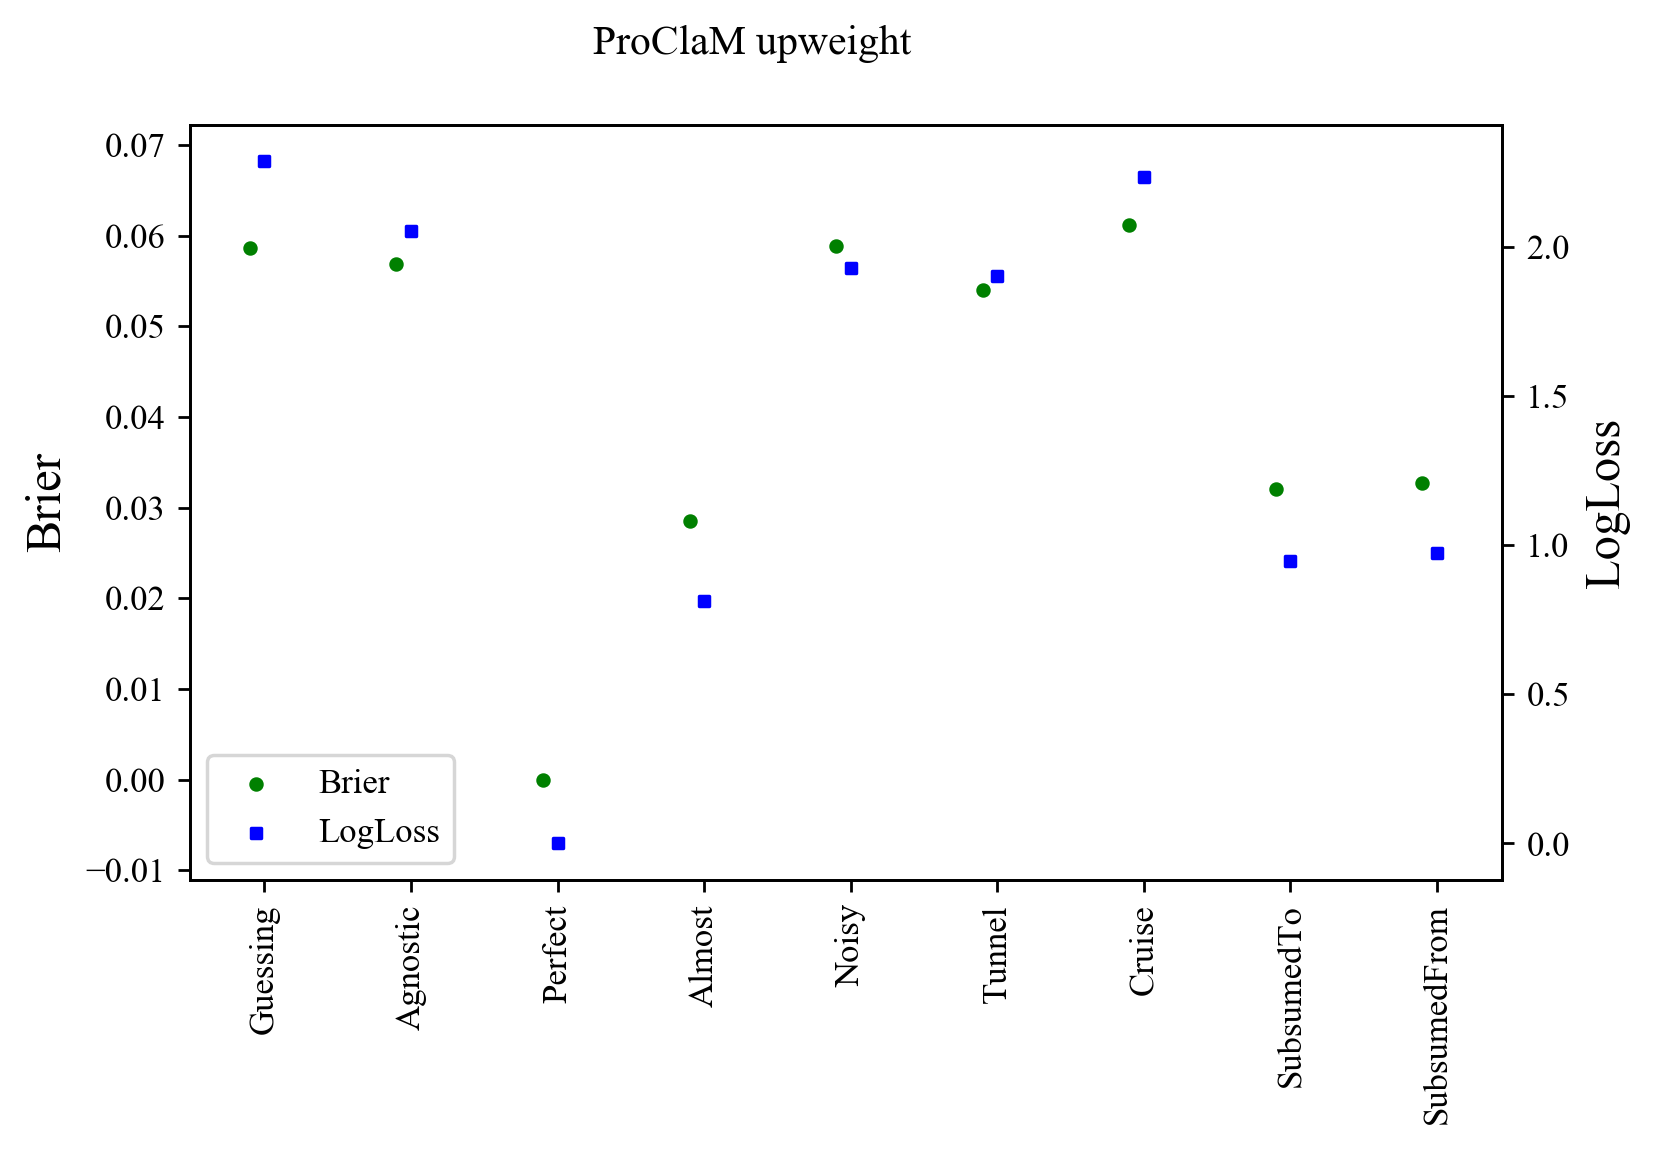
\includegraphics[width=0.5\textwidth]{./fig/multi_metric_up.png}
		\caption{}
		\label{fig:plasticc_up}
	\end{center}
\end{figure}

\subsection{Representative classifications}
\label{sec:realresults}

\begin{figure*}
	\begin{center}
		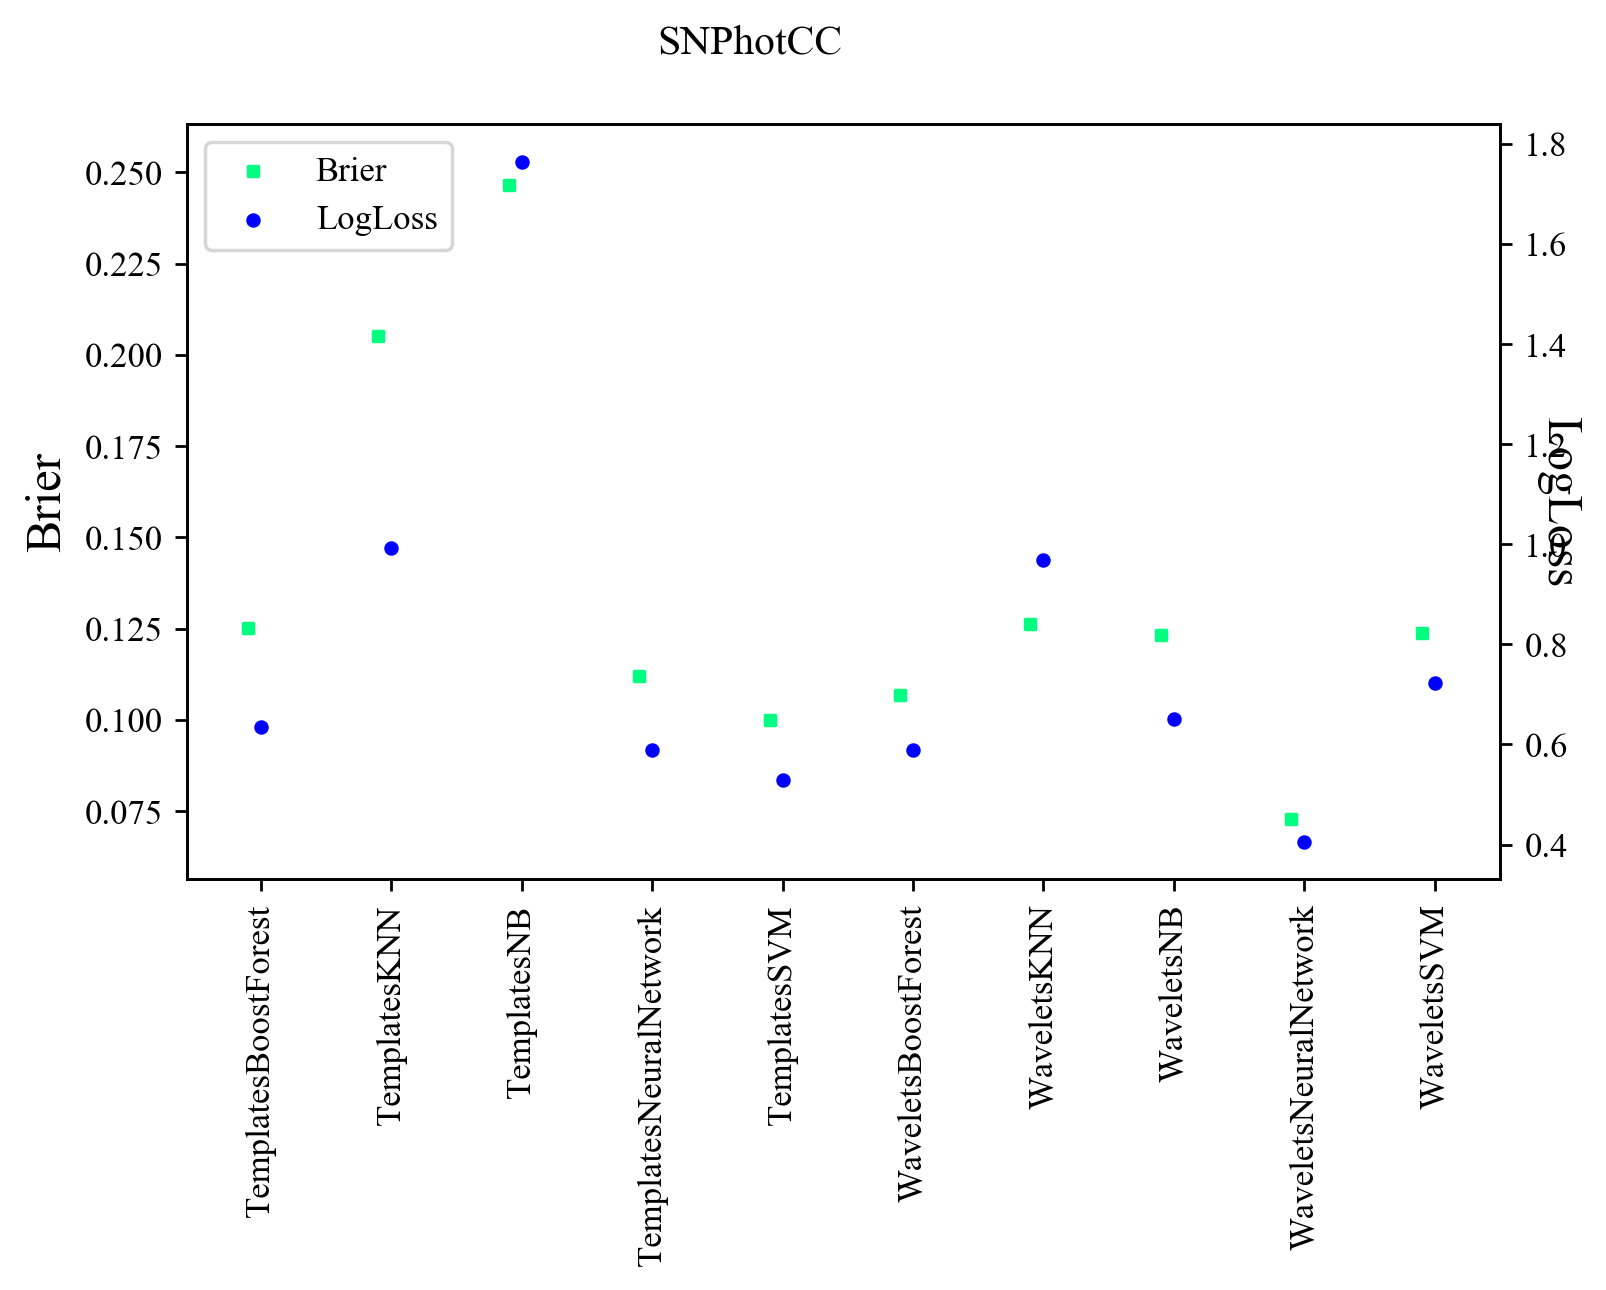
\includegraphics[width=\textwidth]{./fig/SNPhotCC_res.png}
		\caption{}
		\label{fig:snphotcc_metric_compare}
	\end{center}
\end{figure*}

\begin{figure}
	\begin{center}
		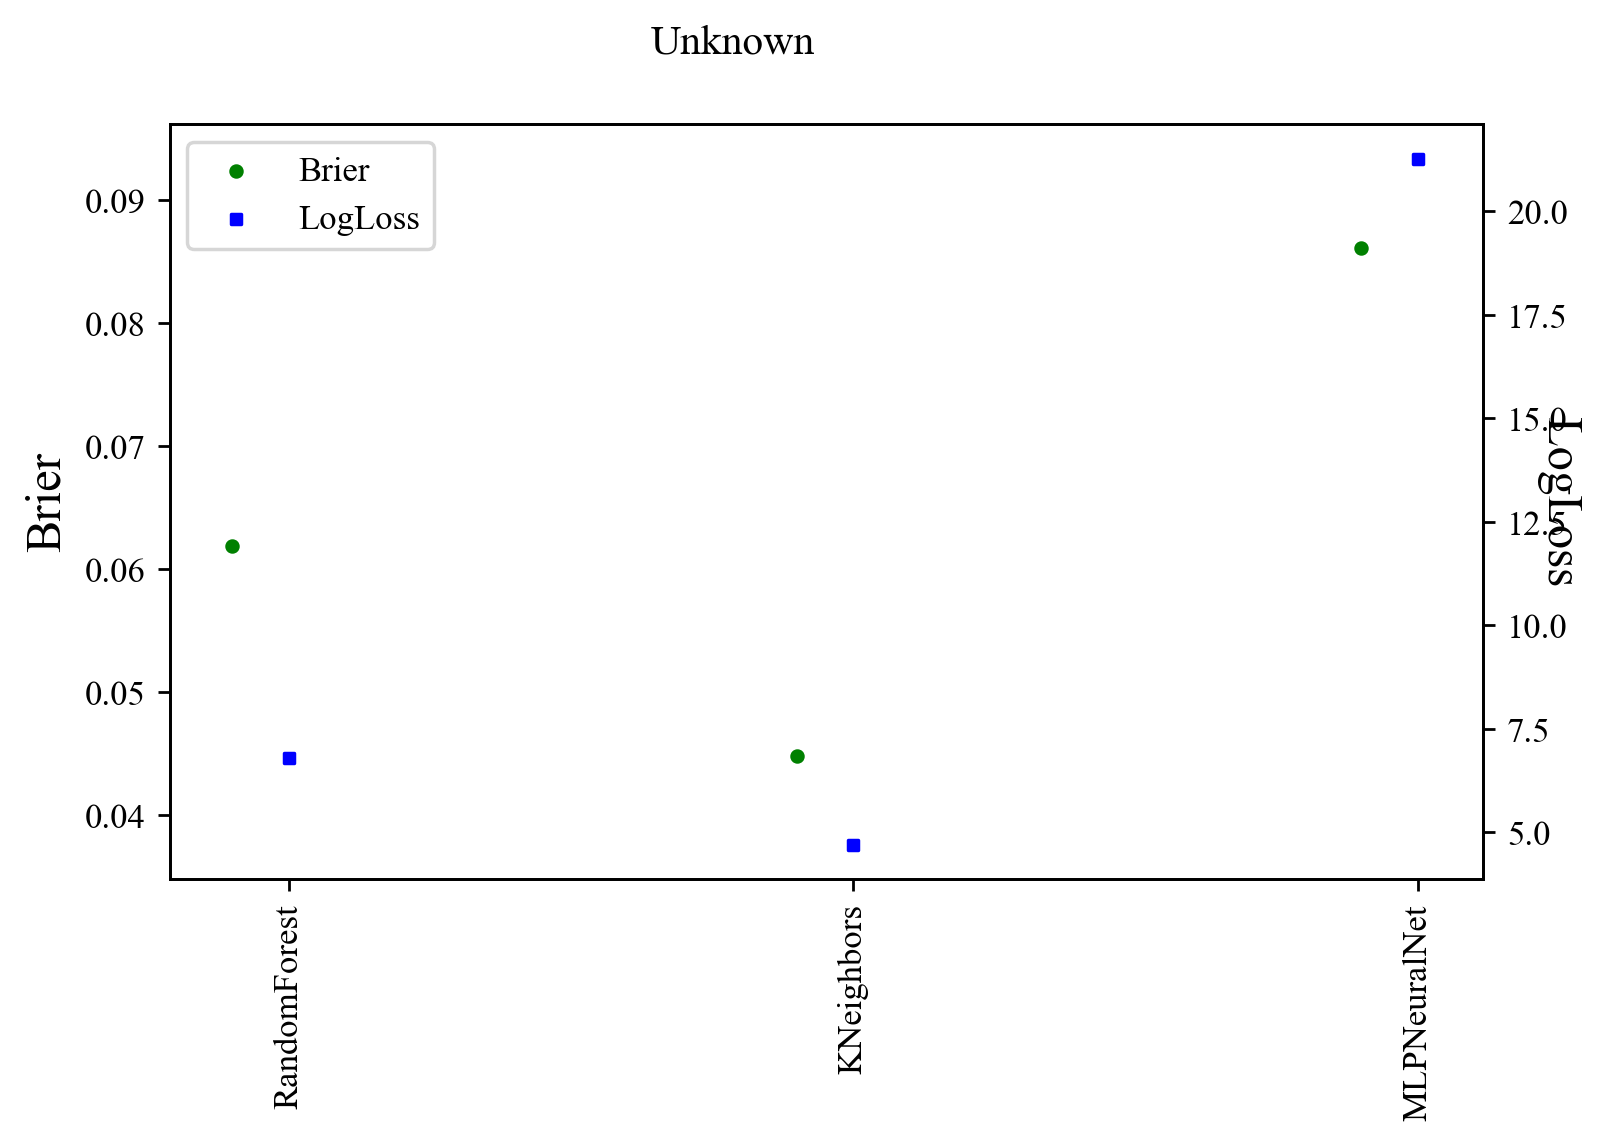
\includegraphics[width=0.5\textwidth,height=5.5in]{./fig/Unknown_res.png}
		\caption{}
		\label{fig:unknown_metric_compare}
	\end{center}
\end{figure}

\subsection{Weighting systematics}
\label{sec:weight_res}

\begin{figure}
	\begin{center}
		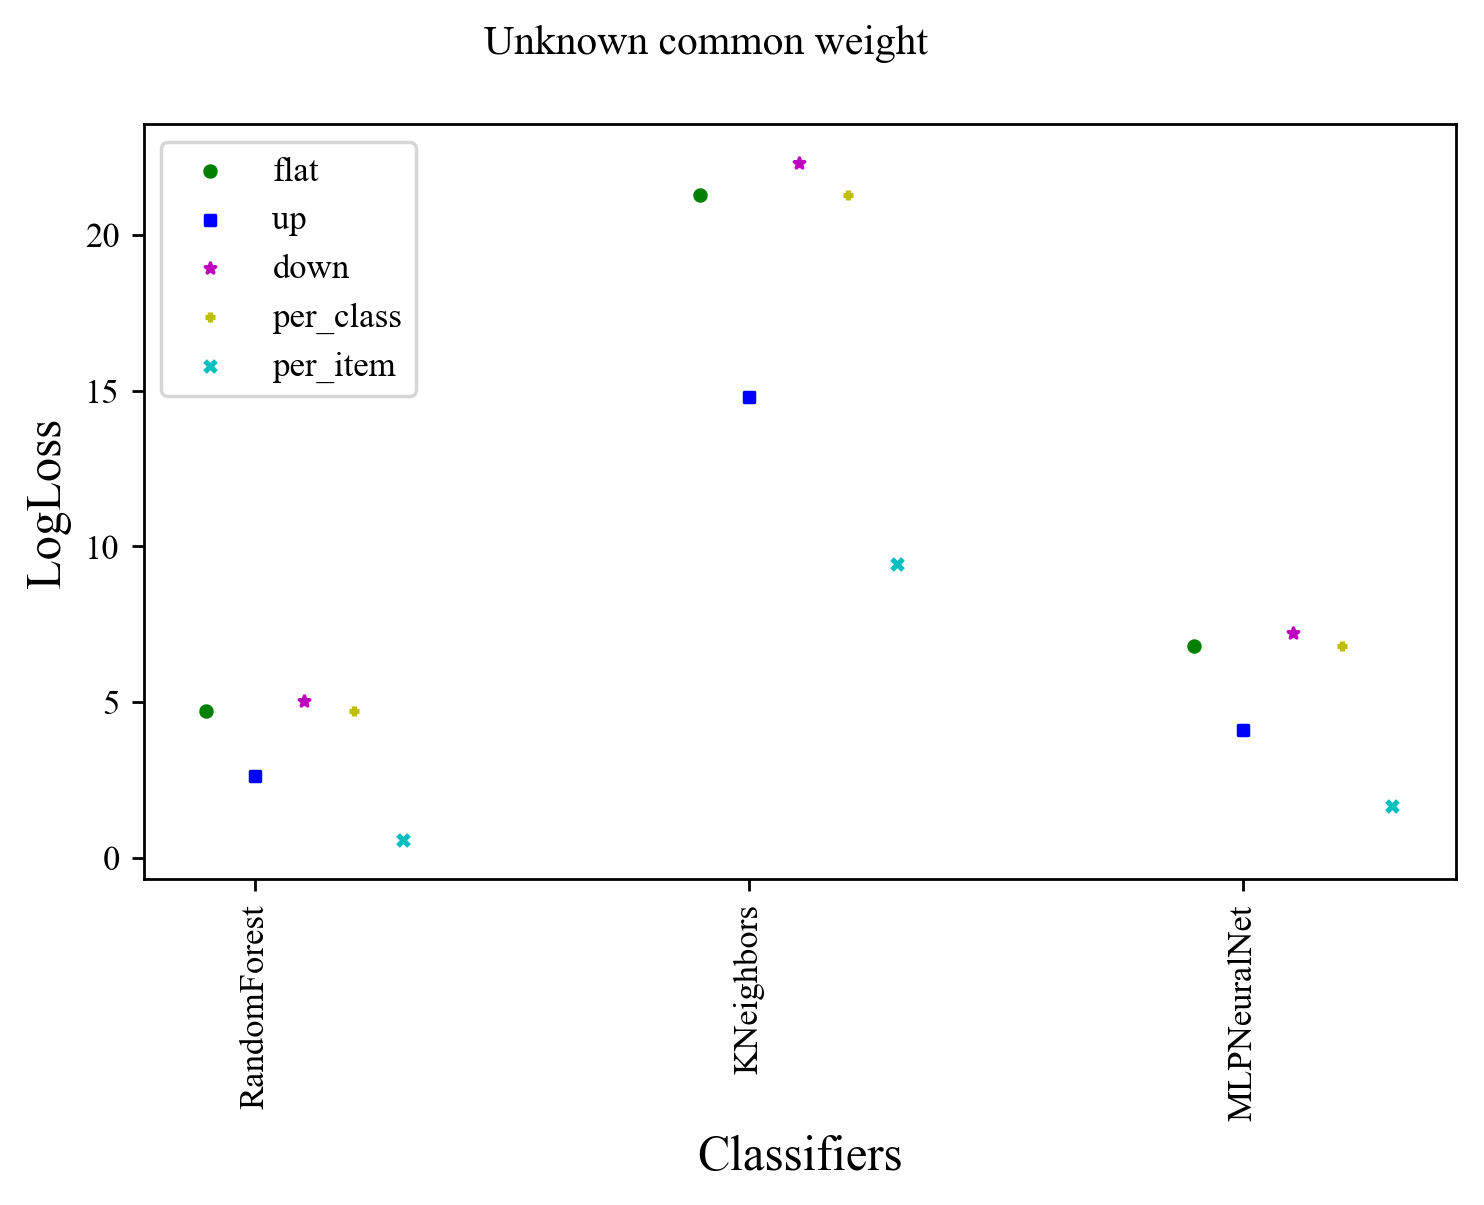
\includegraphics[width=0.5\textwidth]{./fig/systematic_Unknown_common.png}
		\caption{}
		\label{fig:systematic_common}
	\end{center}
\end{figure}

\begin{figure}
	\begin{center}
		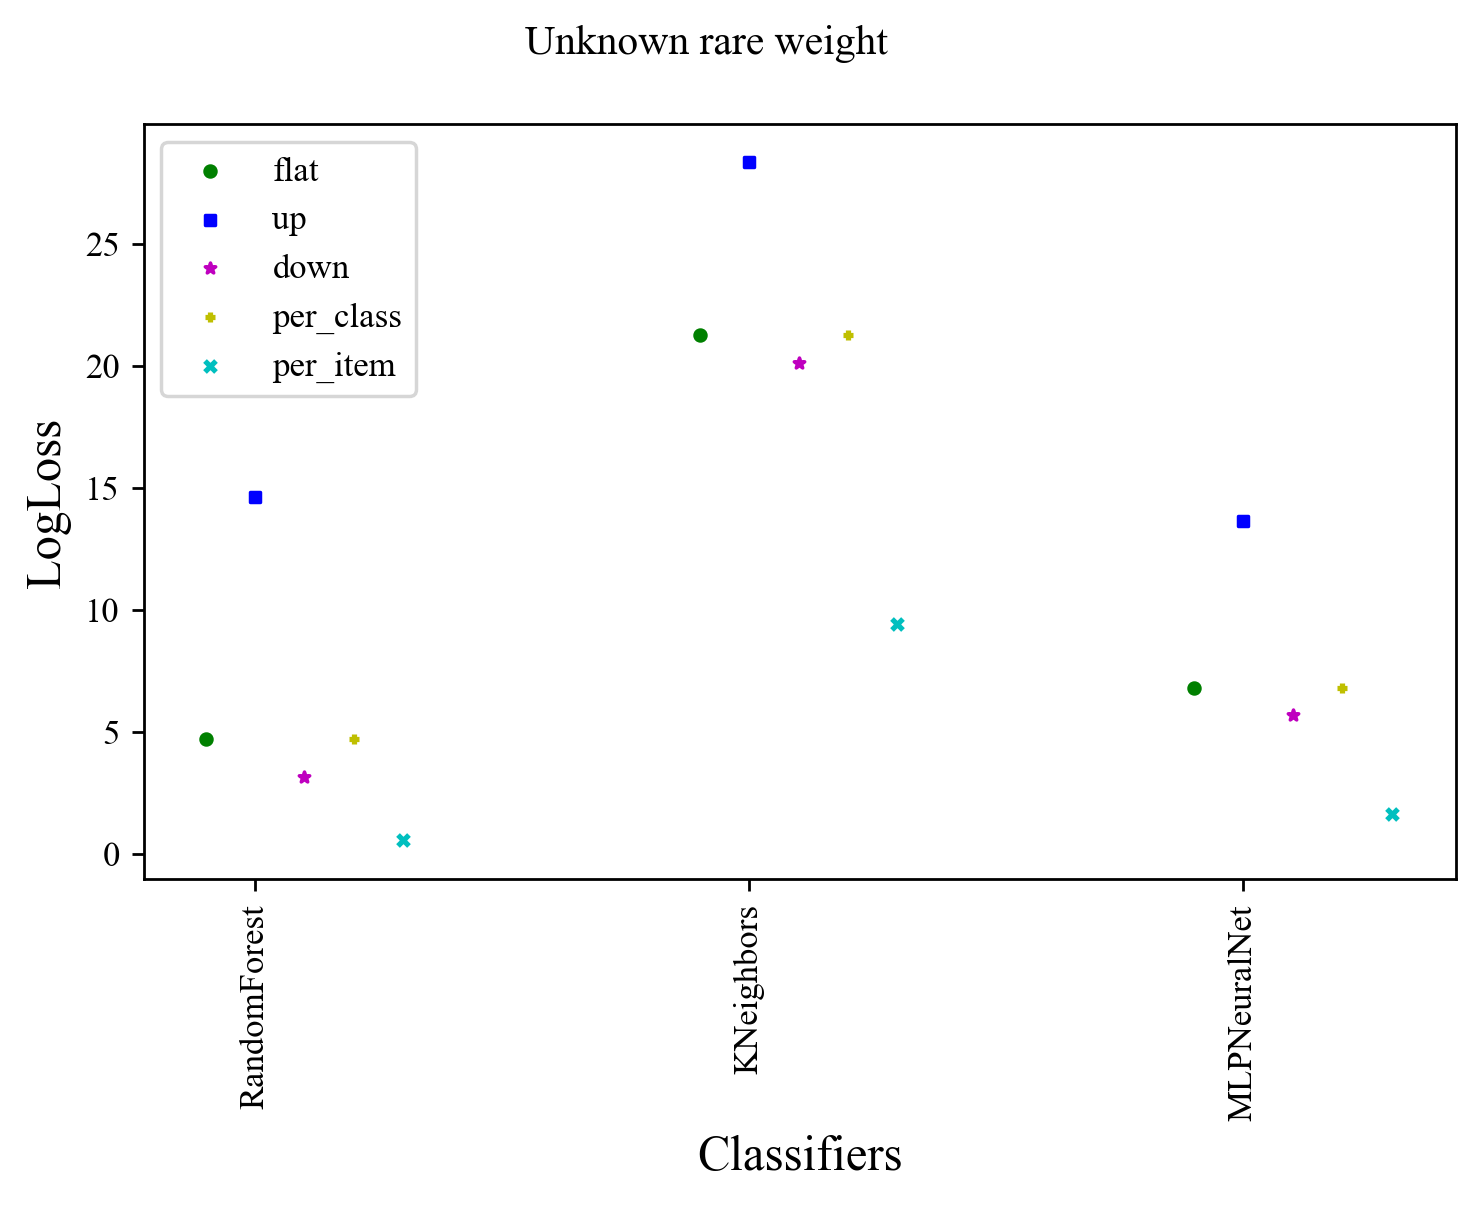
\includegraphics[width=0.5\textwidth]{./fig/systematic_Unknown_rare.png}
		\caption{}
		\label{fig:systematic_rare}
	\end{center}
\end{figure}

\begin{figure}
	\begin{center}
		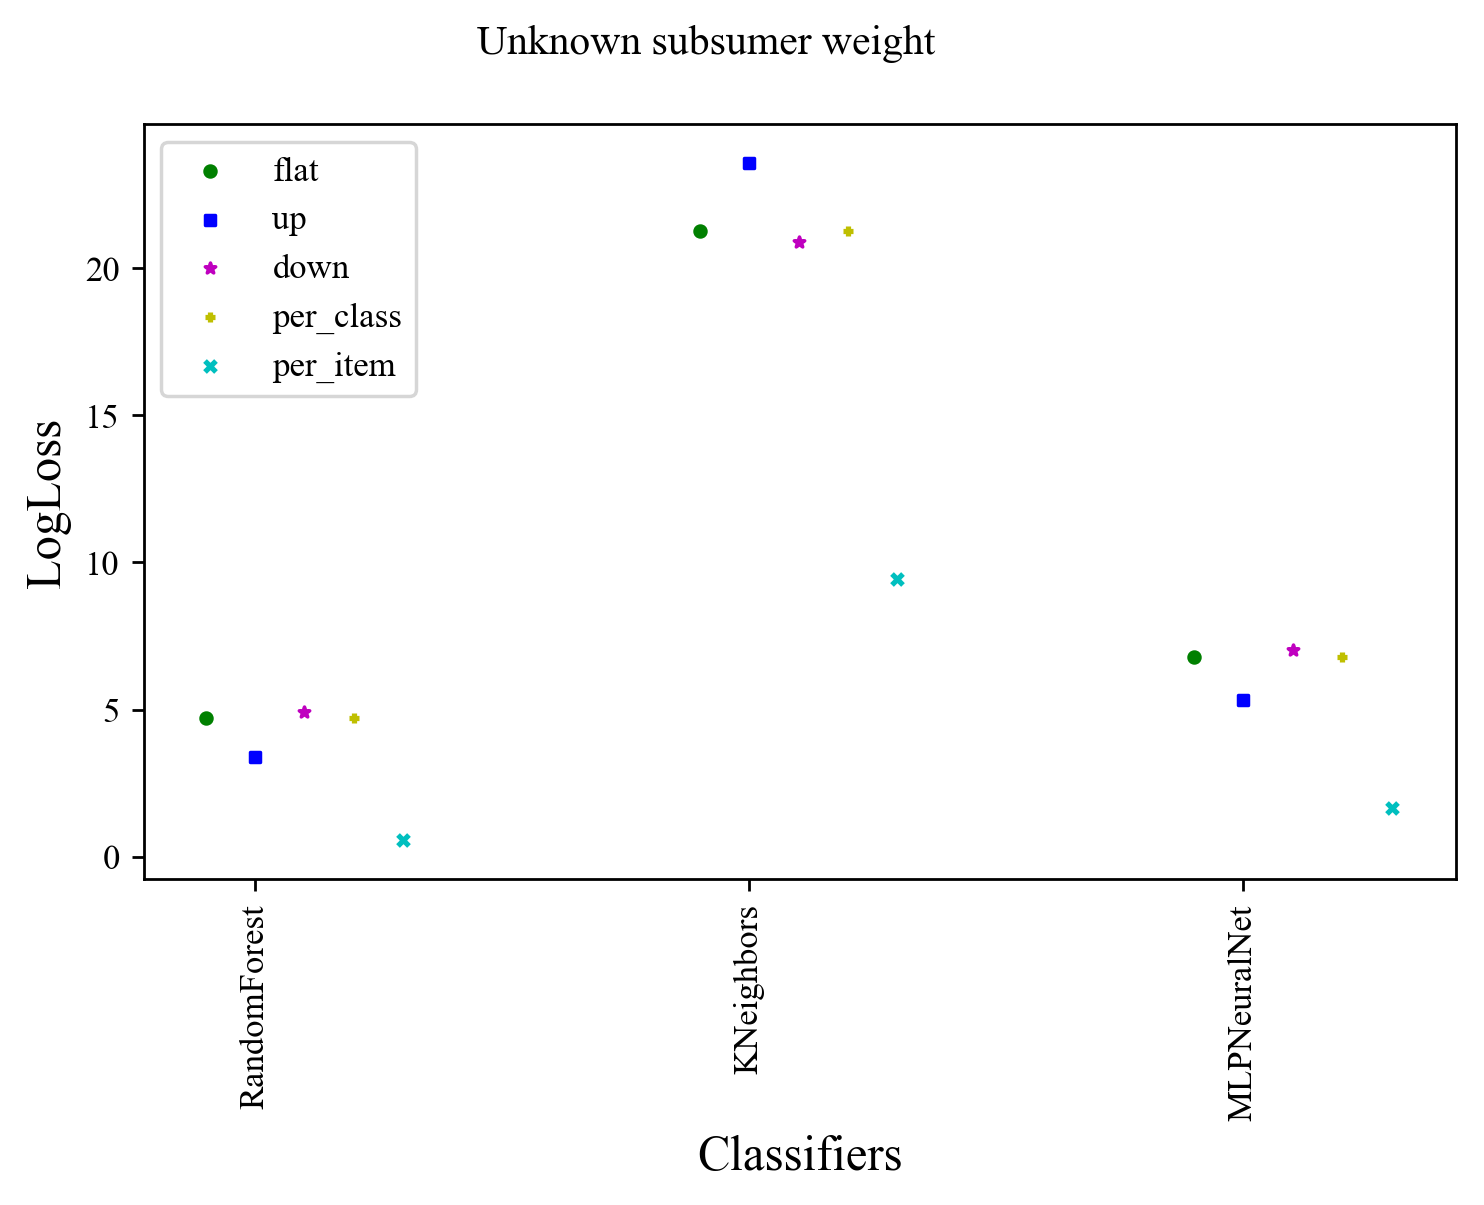
\includegraphics[width=0.5\textwidth]{./fig/systematic_Unknown_subsumer.png}
		\caption{}
		\label{fig:systematic_subsumer}
	\end{center}
\end{figure}

\begin{figure}
	\begin{center}
		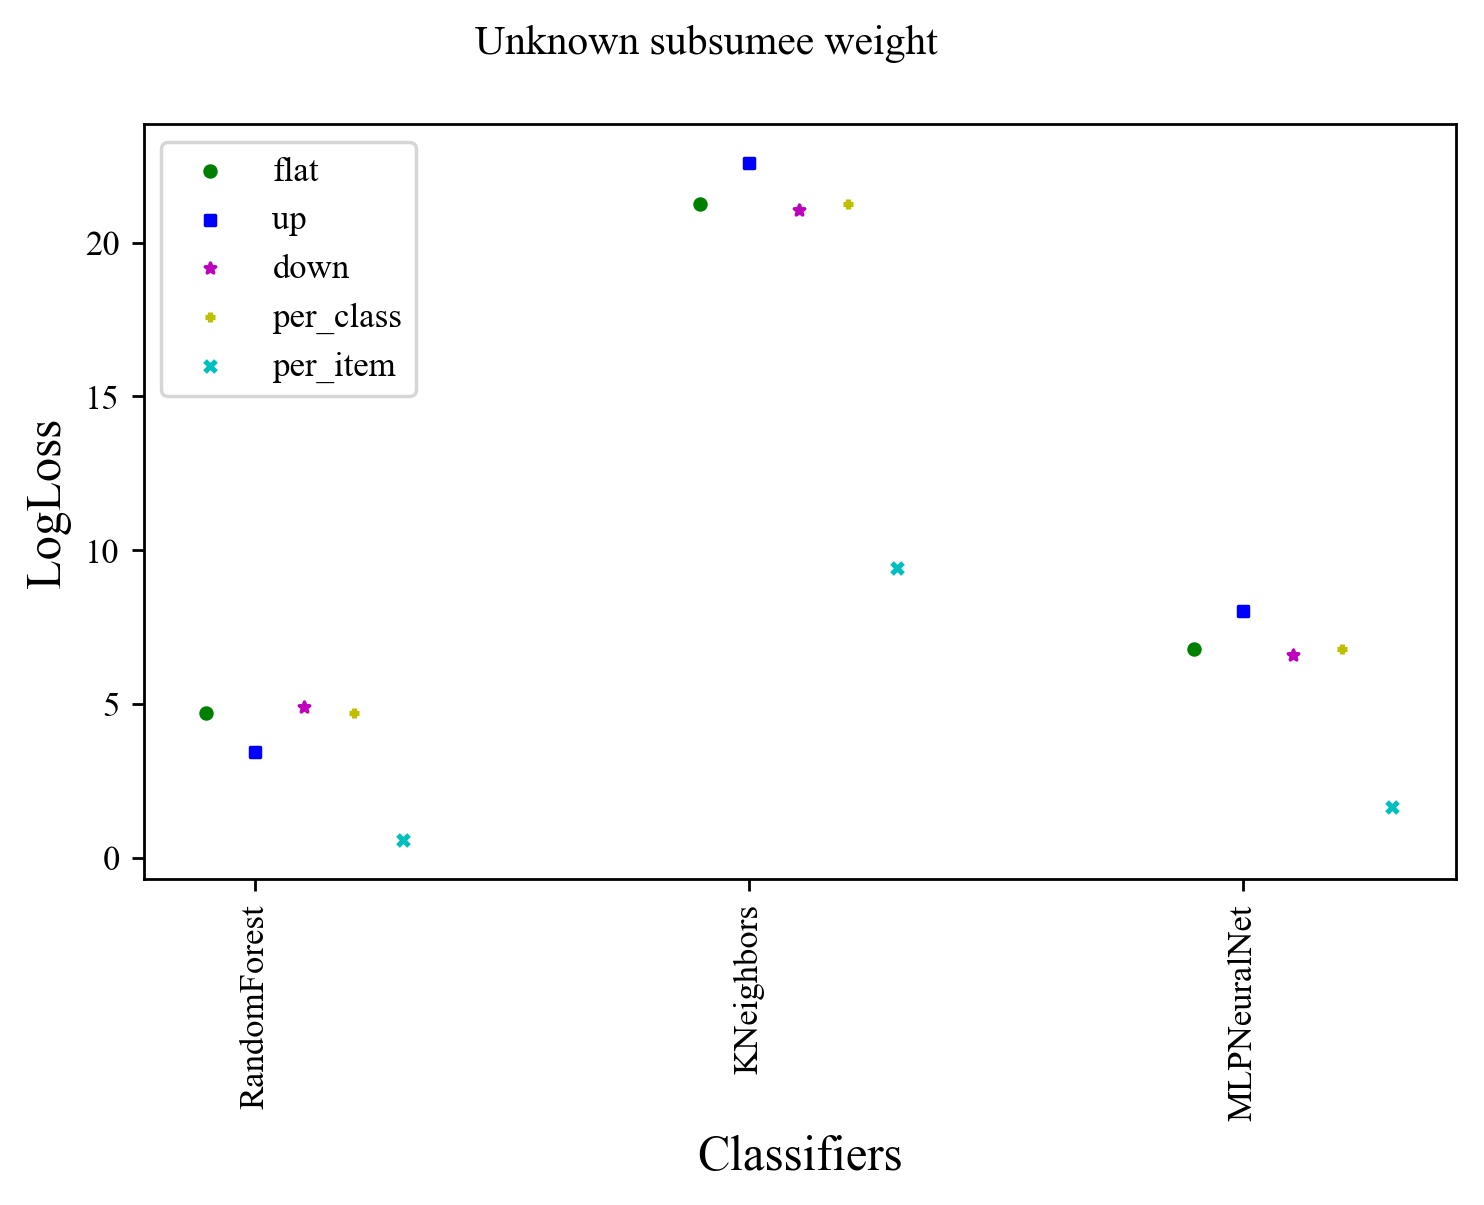
\includegraphics[width=0.5\textwidth]{./fig/systematic_Unknown_subsumee.png}
		\caption{}
		\label{fig:systematic_subsumee}
	\end{center}
\end{figure}

\begin{figure}
	\begin{center}
		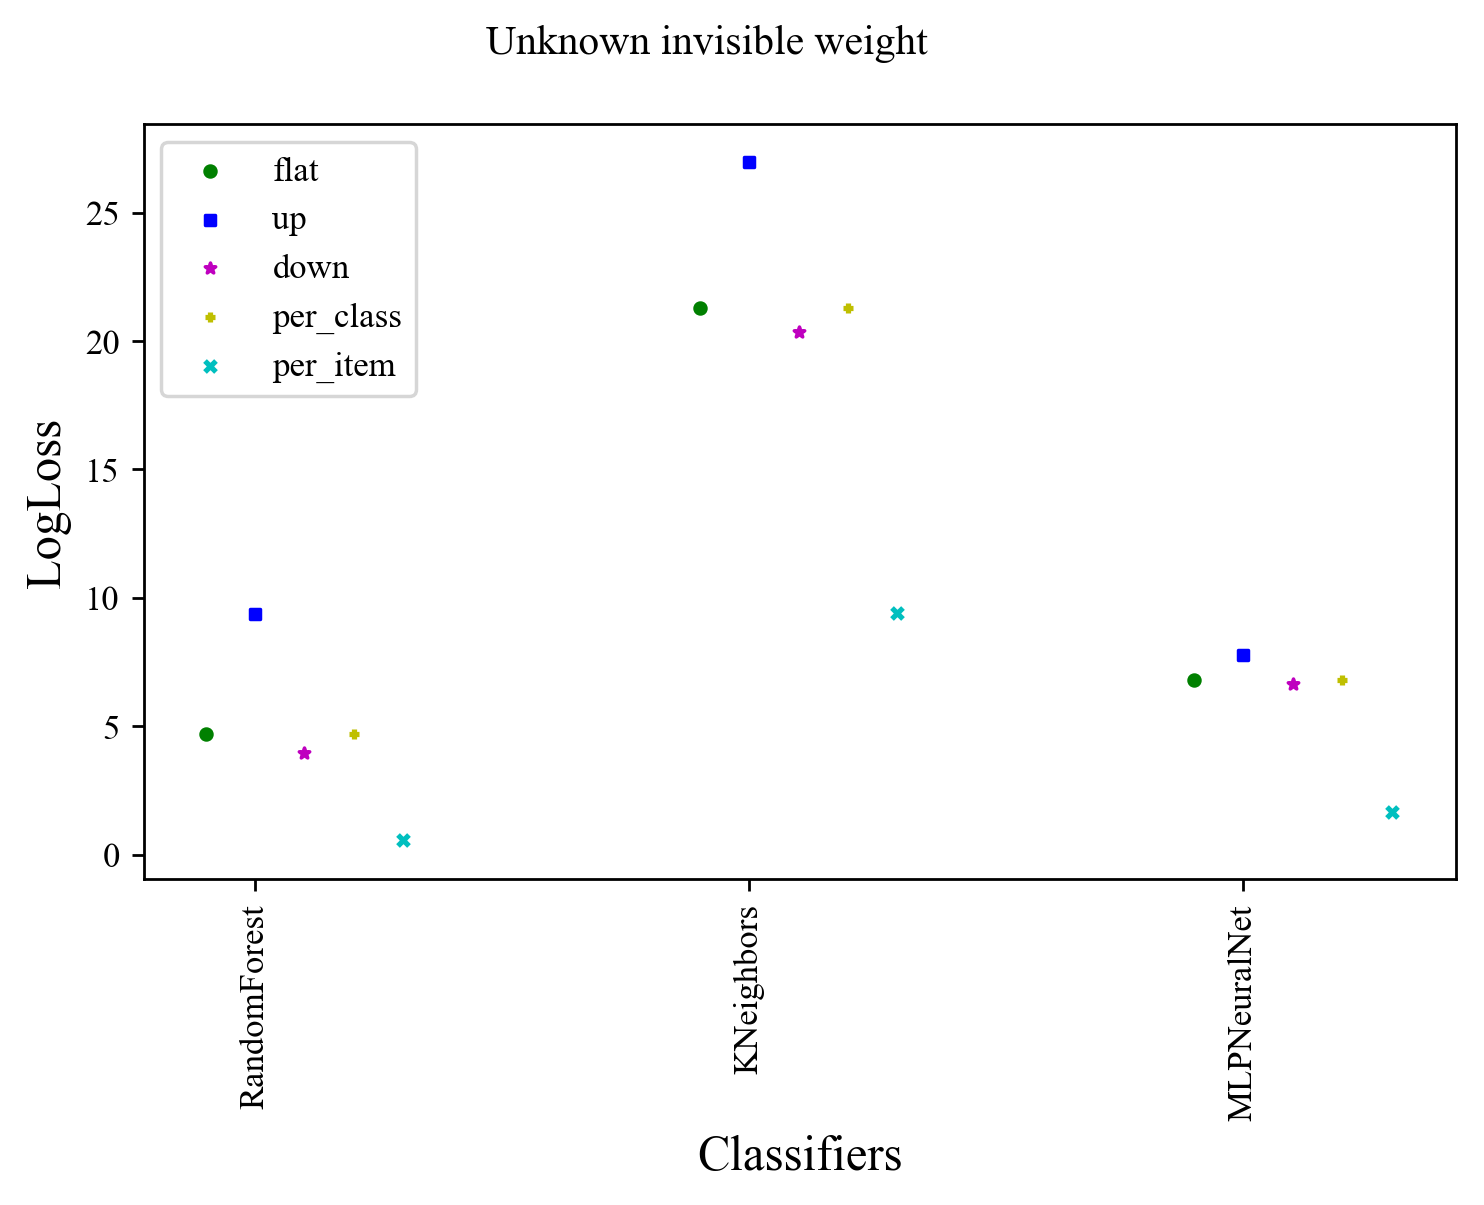
\includegraphics[width=0.5\textwidth]{./fig/systematic_Unknown_invisible.png}
		\caption{}
		\label{fig:systematic_invisible}
	\end{center}
\end{figure}
